%\section*{Summary}
\chapter{Decisions in the real world\clabel{Real}}
In the previous chapter we established the conceptual foundations of ergodicity economics, 
including the formal relationship with expected utility theory, the dominant thinking in economics 
prior to ergodicity economics. We used most of the tools introduced in \cref{Tools}, so from 
here on we can forge ahead and try out some applications. By applications we mean both 
theoretical applications of our new conceptual toolkit, which will allow us to solve theoretical
problems or elicit new aspects of the problems, and we also mean empirical work with data
collected in the lab or in the wild.

In the present chapter we will discuss the early unsystematic observations surrounding the 
St. Petersburg paradox that led to the 
development of expected utility theory; a lab experiment carried out in Copenhagen that puts 
ergodicity economics to the 
test; and we will discuss the surprisingly foundational theoretical problem of insurance: why 
and when do people buy insurance, and how much do they pay for it?

\section{The St. Petersburg paradox}
\seclabel{SPP}
For a bit of history and cultural background, we felt it was a good idea to discuss the 
St. Petersburg paradox, from the perspective of ergodicity economics.

The motivating problem was suggested by Nicolaus 
Bernoulli
%\footnote{Daniel's cousin. 
%The Bernoulli family produced a remarkable 
%number of famous mathematicians in the $17^\text{th}$ and $18^\text{th}$ centuries, 
%who helped lay the foundations of applied mathematics and physics.} 
in 1713 in his 
correspondence with Montmort~\cite{Montmort1713}. 
It involves a hypothetical 
lottery for which the rate of change of expected wealth diverges for any finite ticket 
price. The expected-wealth paradigm would predict, therefore, that people are 
prepared to pay any price to enter the lottery. However, it seems that researchers
in the early 18th century conducted rudimentary informal experiments and presented
the gamble to friends or strangers, asking them how much they'd be willing to wager.
In other words, the expected-wealth paradigm was put to a real-world test. And it failed 
unequivocally: no one wanted to wager more than a few dollars. This is the first 
well-documented example of the inadequacy of the 
expected-wealth paradigm as a model of human decision-making. It was the primary 
motivation for Daniel Bernoulli's and Cramer's development of an alternative model: the
expected-utility paradigm~\cite{Bernoulli1738}. 

It's useful to separate two aspects of the paradox. First, at a superficial level, the divergent
rate of change of expected wealth, irrespective of the fee, may be taken to translate into
the real-world prediction that people will be willing to pay very high prices for a ticket. 
That's not observed, and the prediction is {\it quantitatively wrong}. Second, on a deeper 
level, the entire expected-wealth paradigm fails because it produces no prediction for 
the maximum fee. This quantity diverges under this paradigm -- a good place to remember
that an infinity as a model output is an error message. We will consider the paradox to be
the non-existence of a maximum fee. As we address this core issue, it will turn out that the
quantitative values for this fee are realistic.

In some sense it is a pity that this deliberately provocative and unrealistic lottery has played 
such an important role in the development of classical decision theory.  As we've seen, it is 
quite unnecessary to invent 
a gamble with a divergent change in expected wealth to expose the flaws in the expected-wealth 
paradigm. The presence of infinities in the problem and its variously proposed solutions has 
caused much confusion, and permits objections on the grounds of physical impossibility. These 
objections don't much advance decision theory: they address only the gamble and 
not the decision paradigm. Nevertheless, the paradox is an indelible part not only of history but 
also of the current debate~\cite{Peters2011b}, and so we recount it here. We'll start by defining 
the lottery.

The St. Petersburg lottery requires the player to pay a fee $\F$ and offers a random 
prize whose realisations are power-law distributed, with exponent $-1$. Neither the duration
nor the dynamic are specified in the setup. 

Phrased as a gamble, we have the random payout $\Q$ with realisations 
\be
\forall \gj \in \mathbb{N}^+, \q_{\gj}=\$2^{\gj-1} -\F
\elabel{SPQ}
\ee
and corresponding probabilities 
\be
\p_\gj=\left(\frac{1}{2}\right)^\gj.
\elabel{SPP}
\ee
It's easiest to see the power-law distribution, which causes the divergent first moment, by plotting
$\q_\gj$ vs. $\p_\gj$ on double-logarithmic scales, shown in \fref{SP_power_law} where we've
chosen to set the fee $\F=0$.

\begin{SCfigure}
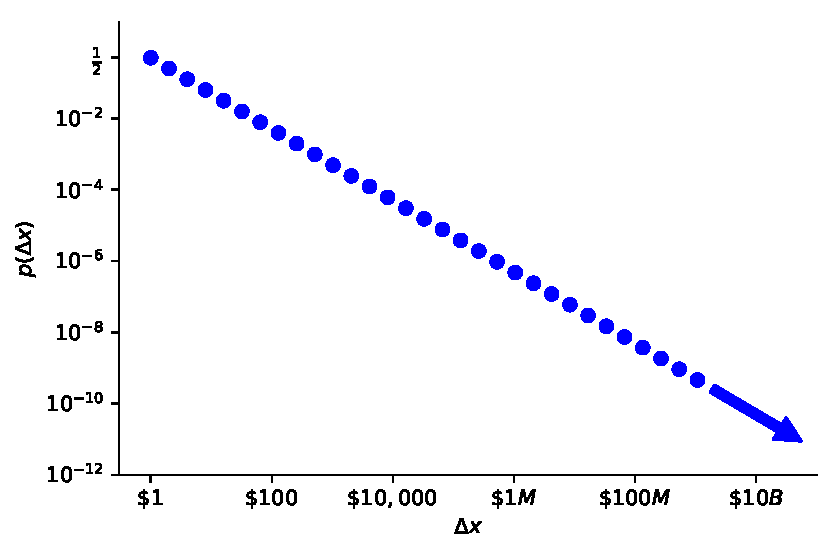
\includegraphics[width=.5\textwidth]{./chapter_real/figs/SP_power_law.pdf}  %\centering
%\begin{picture}(500,110)(0,0)
%  \put(0,0){\includegraphics[width=.3\textwidth]{./gamble.pdf}}
%  \put(150,0){\includegraphics[width=.3\textwidth]{./exp_wealth.pdf}}  
%\put(300,80){C)}
%  \put(300,0){\includegraphics[width=.3\textwidth]{./EUT.pdf}}
%\end{picture}
\caption{The St. Petersburg gamble, at zero fee, defines $(\q_\gj,\p_\gj)$ for all $\gj\in \mathbb{N}^+$, where 
$\q_\gj=\$2^{\gj-1}$, and $\p_\gj(\q_\gj)=\frac{\$1}{2}\q_\gi^{-1}$ decays as a power law with 
exponent $-1$ (the straight line continues indefinitely). This implies a non-existent expectation 
value of $\Q$. Since the expectation value is linear, subtracting any finite fee $\F$ from the possible
prizes still leaves the expectation value of net wealth changes positively divergent.}
\flabel{SP_power_law}
\end{SCfigure}

The problem was considered a paradox because it was posed at a time when the 
expected-wealth paradigm reigned supreme. This means researchers at the time
computed -- or failed to compute -- the expected wealth change $\ave{\D\x}=\ave{\Q}$ 
of the lottery. 
The idea was to compute this as a function of the fee, and find the maximum 
fee people would be willing to pay, that is find 
$\F=\Fmax$ s.t. $\ave{\Q}=0$.

With the random payout $\Q$ specified by \eref{SPQ} and \eref{SPP}, no such fee exists.
The expected wealth change diverges positively for any finite fee. The expected-wealth 
paradigm thus fails, and this precipitated the development of expected-utility theory
in the 18th century.

We will resolve the paradox here via ergodicity 
economics. This is done by specifying the wealth dynamic which we assume the wealth
of a potential player to be subjected to. This is a guess: we would look at the circumstances
of a person and conclude something like ``in the relevant regime his wealth is 
roughly multiplicative'' or whatever dynamic we guess. 
We will then compute the ergodic growth rate corresponding to participation in the lottery, 
and find the value $\Fmax$ at which
this growth rate becomes zero. Since dynamics are generally non-additive, ergodicity 
economics, unlike the expected-wealth paradigm,
does not run aground -- for many realistic dynamics such a fee exists.

Without further ado, here's the solution. We assume multiplicative wealth dynamics
whose ergodic growth rate is $\frac{\D \ln \x}{\D \t}$. The dynamic is not specified
in the problem statement, but neither is a utility function or anything else that would allow
a solution: the problem as stated is underspecified.

Now compute the time average of this growth rate, which we can do by invoking ergodicity
and computing its expectation value.
\be
\frac{\ave{\D \ln \x}}{\D \t}=\frac{\ave{\ln(\x+\q-\F)}-\ln(\x)}{\D\t}.
\elabel{SPg}
\ee
While there's no simple closed-form solution for $\Fmax$, it's not hard to 
show that this expression converges to something finite for sufficiently large fees. 
It also shows us that the time-average growth depends on the player's wealth.
A rich player will be willing to pay a higher fee (though not an arbitrarily 
large fee) than a poor player.

In \fref{gbar_zero} we plot $\Fmax$ (where \eref{SPg} is zero) as a 
function of the player's wealth. These values were obtained numerically.
In the inset we assume a fee of \$2 and plot the time-average growth 
rate \eref{SPg} as a function of the player's wealth. 
\begin{SCfigure}
\centering
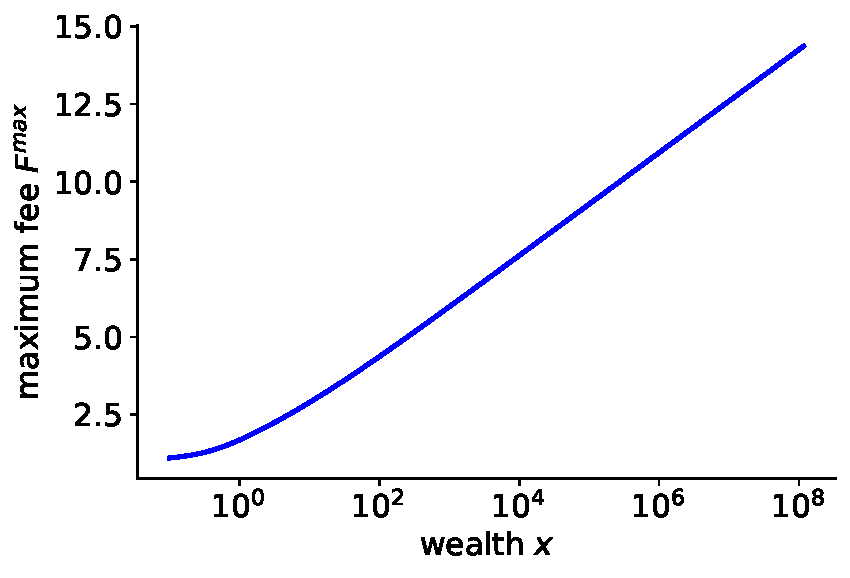
\includegraphics[width=.5\textwidth]{./chapter_real/figs/Fmax.pdf}
\caption{Maximum fee $\Fmax$ which a player is willing to pay {\it vs.} the 
player's wealth $\x$, 
according to ergodicity economics, assuming multiplicative dynamics. 
For a given wealth $\x$, this is the value of $\F$ where the time-average of the ergodic 
growth rate \eref{SPg} is zero. This 
resolves the 300-year old paradox because for any finite $\x$ a finite $\Fmax$ exists. 
Adapted from~\cite{Peters2011b}.\flabel{gbar_zero}}
\end{SCfigure}

%\begin{figure}
%\centering
%\begin{picture}(200,230)(0,0)
%\put(-75,0){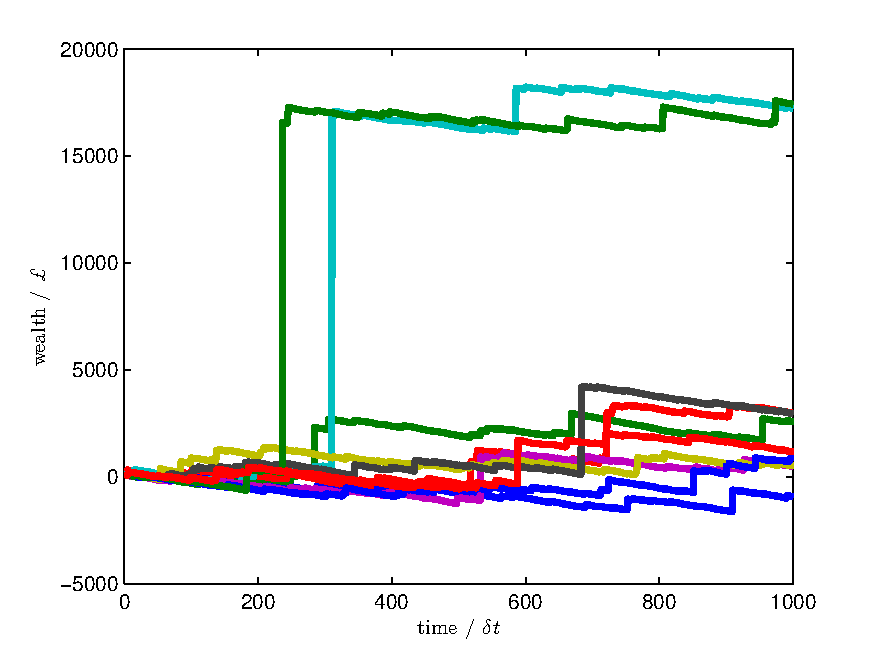
\includegraphics[width=\textwidth]{./chapter_riskless/figs/lottery_add_traj.pdf}}
%\end{picture}
%\caption{Wealth trajectories for the additively repeated St Petersburg lottery, 
%with starting wealth, $\x(0)=\$100$, and ticket price, $\F=\$10$. 
%Ten trajectories are plotted over 1,000 rounds.\flabel{lottery_add_traj}}
%\end{figure}
Treatments based on multiplicative repetition have appeared sporadically in the 
literature, starting with Whitworth in 
1870~\cite[App.~IV]{Whitworth1870}.\footnote{Whitworth was dismissive of early 
utility theory: ``The result at which we have arrived is not to be classed with 
the arbitrary methods which have been again and again propounded to evade 
the difficulty of the Petersburg problem\ldots. Formulae have often been proposed, 
which have possessed the one virtue of presenting a finite result\ldots but they 
have often had no intelligible basis to rest upon, or\ldots sufficient care has not 
been taken to draw a distinguishing line between the significance of the result 
obtained, and the different result arrived at when the mathematical expectation 
is calculated.'' Sadly he chose to place these revolutionary remarks in an appendix 
of a college probability textbook.} It is related to the famous Kelly 
Criterion~\cite{Kelly1956}\footnote{Kelly was similarly unimpressed with the 
mainstream and noted in his treatment of decision theory, which he developed 
from the perspective of information theory and which is identical to ergodicity 
economics with multiplicative dynamics, that the utility function is ``too general 
to shed any light on the specific problems of communication theory.''}, although 
Kelly did not explicitly treat the St Petersburg game, and tangentially to \Ito's 
lemma~\cite{Ito1944}. It appears as an exercise in a well-known text on information 
theory~\cite[Ex.~6.17]{CoverThomas1991}. Mainstream economics has ignored all 
this. A full and rigorous resolution of the paradox, including the epistemological 
significance of the shift from ensemble to time averages, was published recently 
by one of the present authors~\cite{Peters2011b}.

%
%Imagine a starting prize 
%of $\$1$ (originally the prize was in ducats). A fair coin is tossed: 
%if it lands heads, the player wins the prize and the lottery ends; if it lands 
%tails, the prize is doubled and the process is repeated. Therefore, the 
%player wins $\$2$, $\$4$, $\$8$ if the first head lands 
%on the second, third, fourth toss, and so on. The player must buy a ticket, 
%at price $\F$, to enter the lottery. The question is: what is 
%the largest $\F$ the player is willing to pay?
%
%The lottery can be translated neatly into our gamble formalism:
%\be
%\q_\gj = \$ 2^{\gj-1} - \F, \quad \p_\gj = 2^{-\gj},
%\elabel{lottery_def}
%\ee
%for $\gj\in\{1,2,3,\ldots\}$, \ie the set of positive integers. The vast majority 
%of observed payouts are small, but occasionally an extremely large payout 
%(corresponding to a very long unbroken sequence of tails in the classical 
%description) occurs. This is shown in the example trajectories in 
%\fref{lottery_add_traj}, where the lottery has been repeated additively.
%
%From now on we will forget about the coin tosses, which are simply a 
%mechanism for selecting one of the possible payouts. They 
%are nothing but an 18th-century random number generator. Instead we shall work with the 
%compact definition of the lottery in \eref{lottery_def} and assume it 
%takes a fixed amount of time, $\dt$, to play.
%
%The rate of change of expected wealth is
%\bea
%\frac{\ave{\d\x}}{\dt} & = & \frac{1}{\dt} \sum_{\gj=1}^\infty \p_\gj \q_\gj \\
%&=& \frac{1}{\dt} \left( \$ \sum_{\gj=1}^\infty 2^{-\gj}\,2^{\gj-1} - \sum_{\gj=1}^\infty 2^{-\gj} \F \right) \\
%&=& \frac{1}{\dt} \left( \$ \sum_{\gj=1}^\infty \frac{1}{2} - \F \right). \elabel{lottery_ex_wealth}
%\eea
%This diverges for any finite ticket price. Under the expected-wealth paradigm, 
%this means that the lottery is favourable at any price.

%
%This implausible conclusion, which does not accord with human behaviour, 
%exposes the weakness of judging a gamble by its effect on expected 
%wealth. Daniel Bernoulli suggested to resolve the paradox by adopting 
%the expected-utility paradigm. His choice of utility function was the 
%logarithm, $\gu(\x)=\ln \x$, which, as we now know, produces a decision 
%rule equivalent to growth-rate optimisation under multiplicative repetition. 
%This correspondence was not appreciated by Bernoulli: indeed 
%$18^\text{th}$-century mathematics did not possess the concepts and 
%language required to distinguish between averages over time and across 
%systems, even though it had the basic arithmetic tools. 
%%In any case, the 
%%correspondence relies on the choice of a particular utility function, and vanishes the moment something other than the logarithm is chosen. We also have
%%to interpret expected utility theory a little differently from how it is usually presented -- for instance we have to assume that expected changes in utility really mean expected rates of changes, with a specific gamble duration, \ie we have to introduce the concept of time into utility theory quite differently from that's usually done (which we won't discuss here).
%
%Unfortunately, Bernoulli made a mathematical error in the implementation 
%of his own paradigm -- accidentally he proposed two mutually inconsistent 
%versions of utility theory in the paper that established the paradigm. Initially, 
%the error had little impact, and it was corrected by Laplace in 
%1814~\cite{Laplace1814}. But Laplace didn't openly say he'd corrected an 
%error, he just worked with what he thought Bernoulli had meant. This politeness 
%had awful consequences. In 1934 Menger~\cite{Menger1934}, keen to get the 
%story right, went back to the original text by Bernoulli. He didn't notice the 
%error but rather got confused by it which led him to introduce a further error. 
%Based on this car crash of scientific communication, Menger derived the 
%infamous (wrong) claim we encountered in the history segment in \secref{dyn_from_u}: utility functions 
%must be bounded, with disastrous consequences for the budding neoclassical formalism. We 
%will leave this most chequered part of the paradox's history alone -- details can be found 
%in~\cite{PetersGell-Mann2016,Peters2019}. Instead we will focus on what's usually 
%presumed Bernoulli meant to write.
%
%\begin{example}{Resolution by logarithmic utility}
%Instead of \eref{lottery_ex_wealth}, we calculate the rate of change of expected logarithmic utility,
%\bea
%\frac{\ave{\d\ln \x}}{\dt} & = & \frac{1}{\dt} \sum_{\gj=1}^\infty \p_\gj \left[\ln(\x+\q_\gj)-\ln \x\right] \\
%&=& \frac{1}{\dt} \sum_{\gj=1}^\infty 2^{-\gj} \ln\left(\frac{\x+\$2^{\gj-1}-\F}{\x}\right), \elabel{lottery_ex_util}
%\eea
%where $\x$ is the ticket buyer's wealth.
%
%This is finite for all finite ticket prices less than the buyer's wealth plus the smallest 
%prize: $\F<\x+\$1$. This can be shown by applying the ratio 
%test.\footnotemark\ It may be positive or negative, depending on the values 
%of $\F$ and $\x$. \fref{gbar_zero} shows the locus of points in the $(\x,\F)$-plane 
%for which the sum is zero.
%\end{example}
%\footnotetext{The ratio of the $(\gj+1)^\text{th}$ term to the $\gj^\text{th}$ term 
%in the sum tends to $1/2$ as $\gj\to\infty$.}
%
%The utility paradigm is a model that resolves the paradox, in the sense that creates 
%a world where players may decline to buy a ticket. Bernoulli argued for this resolution 
%framework in plausible terms: the usefulness of a monetary gain depends on how 
%much money you already have. He also argued specifically for the logarithm in 
%plausible terms: the gain in usefulness should be proportional to the fractional gain 
%it represents, $\d \gu = \d\x/\x$. Yet, the framework has left many unsatisfied: why 
%does usefulness have this functional form? We provide this deeper reason by 
%connecting the problem to dynamics and time, unlike Bernoulli. Had Bernoulli made 
%the connection, he might have been less willing to accept Cramer's square-root utility 
%function as an alternative, which, as we've seen, corresponds to a rather less intuitive dynamic.
%
%%However, while plausible, the framework relies on a utility function, which must be postulated. It can neither be derived from fundamental considerations nor verified empirically.
%
%Turning to our decision algorithm, we will assume that the lottery is assessed by
%the growth rate it would impart on the player were it repeated 
%multiplicatively. This means, in effect, that the prizes and ticket price are treated 
%as fractions of the player's wealth, such that the effect of each lottery is to 
%multiply current wealth by a random factor,
%\be
%\gr_\gj = \frac{\x+\$2^{\gj-1}-\F}{\x}, \quad \p_\gj= 2^{-\gj}.
%\ee
%This follows precisely our earlier treatment of a gamble with multiplicative dynamics, 
%and we can apply our results directly. The time-average (exponential) growth rate is
%\be
%\gt_\text{m} = \frac{1}{\dt} \lim_{\T\to\infty} \left\{ \frac{1}{\T}  \sum_{\gtau=1}^\T \ln \gr(\gtau) \right\} = \frac{1}{\dt}  \sum_{\gj=1}^\infty 2^{-\gj} \ln \gr_\gj, \elabel{lottery_gbar}
%\ee
%which is identical to the expression for the rate of change of expected log-utility, 
%\eref{lottery_ex_util}. This is, as we've discussed, because $\gv(\x)=\ln(\x)$ 
%is the appropriate ergodicity transformation for multiplicative dynamics. The result is the same, but 
%the interpretation is different: we have assumed less, only that our player is 
%interested in the growth rate of his wealth and that he gauges this by imagining 
%the outcome of an indefinite sequence of repeated lotteries.
%
%Thus the locus in \fref{gbar_zero} also marks the decision threshold \textit{versus} 
%the null gamble under our decision axiom. The player can sensibly decline the 
%gamble, even though it results in a divergent change in expected wealth. This 
%is illustrated by comparing \fref{lottery_mult_traj}, which shows trajectories of 
%multiplicatively repeated lotteries, with the additively repeated lotteries already 
%seen in \fref{lottery_add_traj}.
%\begin{figure}
%\centering
%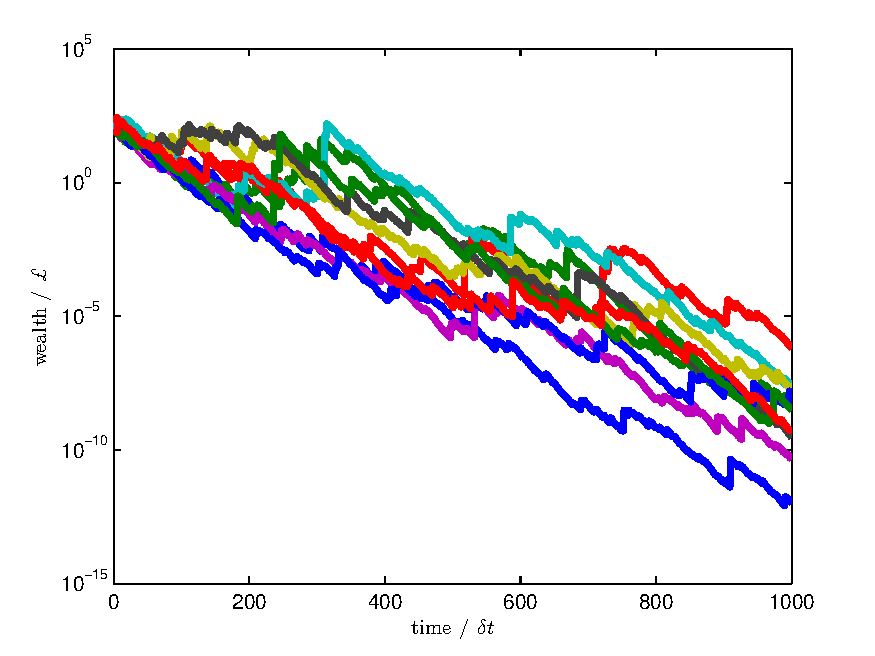
\includegraphics[width=\textwidth]{./chapter_riskless/figs/lottery_mult_traj.pdf}
%\caption{Wealth trajectories for the multiplicatively repeated St Petersburg lottery, 
%with starting wealth, $\x(0)=\$100$, and ticket price, $\F=\$10$. Ten 
%trajectories are plotted over 1,000 rounds. The realisations of the individual 
%lotteries are the same as in \fref{lottery_add_traj} but the mode of repetition is 
%different.\flabel{lottery_mult_traj}}
%\end{figure}
%The trajectories are based on the same sequences of lottery outcomes, only 
%the mode of repetition is different. The simulation shows us visually what we 
%have already gleaned by analysis: what appears favourable in the 
%expected-wealth paradigm (corresponding to additive repetition) results in a 
%disastrous decay of the player's wealth over time under a realistic dynamic.
%
%As $\F\to \x+\$1$ from above in \eref{lottery_gbar}, $\gt_\text{m}$ diverges 
%negatively, since the first term in the sum is the logarithm of a quantity approaching 
%zero. This corresponds to a lottery which can make the player bankrupt. The effect 
%is also shown in the inset of \fref{gbar_zero}.
%


\section{The Copenhagen experiment}
At the end of \secref{Expected_utility} we arrived at a mapping between expected utility 
theory and ergodicity economics. The fact that such a mapping is possible is fascinating: careful 
thinking leads to almost identical mathematical expressions, whether we operate in the conceptual
universe of 1738 or in that of today. Since the difference is first and foremost conceptual, 
it is fair to ask whether ergodicity economics is just another way of looking at the subject
without fundamentally different or new results. That alone would be a wonderful achievement,
as Rota put it when speaking about exterior algebra \cite[p.48]{Rota} [indiscrete thoughts]: 
%``You are right. There is nothing in yesterday's mathematics that you can prove with exterior algebra that could not
%also be proved without it. Exterior algebra 
``[It] is not meant to prove old facts, it is meant to disclose a new world. Disclosing new 
worlds is as worthwhile a mathematical enterprise as proving old conjectures.''

But we will see that the new world disclosed by ergodicity economics does more than 
prove old conjectures. Our first expeditions into this new world have revealed rich 
new lands and call for further ships to be sent out to sea.

So: different concepts, very nice. But do the differences between concepts allow an experiment, 
at least in principle, that would tell us something radically new. Specifically, since we can 
map ergodicity economics and expected utility theory under certain conditions, can an experiment
be designed that has discriminating power between the two mapped models? If we mess with the
conditions that allow the mapping, so that the two models are no longer equivalent, which model
will be better at describing observed behaviour?

Without our knowledge, a group of neuroscientists at the Danish Research Center for Magnetic 
Resonance in Copenhagen was asking precisely this question.

They followed very closely the discussion in \cite{PetersGell-Mann2016}, where we had worked 
out in detail the correspondences between linear utility and additive dynamics; and between 
logarithmic utility and multiplicative dynamics. These correspondences provide the basis for 
the experiment: what if the dynamics of wealth could be controlled? With two artificial 
environments -- one additive,  one multiplicative -- do people adjust their behaviour to be 
growth-optimal in each? That's the basic idea: observe the choices that people make under
different wealth dynamics, and infer from those choices the ergodic growth rate (or utility 
function) that is being optimised.

A positive result -- people changing their utility functions in response to the dynamics -- would falsify 
expected utility theory (insofar as experiments falsify models). In the worldview of expected 
utility theory, the utility function encodes a personality. Supposedly, it's a psychological or 
even neurological property of a human being, and not something that can change over the 
course of a few hours (the duration of the experiment). 

A negative result -- people not changing utility functions -- would get ergodicity economics into trouble 
(at least in this experiment). In the worldview of ergodicity economics, the term ``utility function'' 
is a poorly chosen label for what's really the ergodicity transformation that sits in the functional 
form of the relevant growth rate. This transformation is different for these two dynamics, as we've 
seen. And the postulate of ergodicity economics is that people behave so as to optimise the 
rate of change of the ergodicity transformation (\ie the ergodic growth rate). If they keep using the 
same transformation, irrespective of dynamics, then this postulate would 
not describe real behaviour.

As we discuss the experiment below, we have to keep its limitations in mind. Of course, 
we could set up a flawed experiment. We could have a bug in the code to analyse the 
observations and accidentally introduce spurious differences between the inferred utility functions. 
Or we could set up an experiment that doesn't achieve statistical significance to fish out 
of the noise the relevant differences in the ergodicity mappings that people optimise. 
Such experiments would not falsify anything; they would just be invalid. 

The experiment is described in detail in \cite{MederETAL2019}. Here we will only outline the setup. 
In the additive environment the subject was given a starting wealth of about \$150 and then 
made 312 choices of the (additive) form ``would you rather toss a coin for winning \$40 or losing 
\$30; or for winning \$30 or losing \$20?'' 

In the multiplicative environment, the same subject was also given about \$150, and then made 
312 choices of the (multiplicative) form ``would you rather toss a coin for a 100\% gain in wealth 
or a 70\% loss; or for a 30\% gain or a 20\% loss?''

The choices were consequential: a single decision could lead to winning or losing several 
hundred real dollars. 
%Test subjects were selected not to have received quantitative training -- no physicists or mathematicians were allowed to participate, and all manner of controls were carried out. For instance, one group gambled under additive dynamics first, the other under multiplicative dynamics.

We won't go into the details of the data analysis, which is rather sophisticated in this case. Instead, 
we will only explain the logic behind what was done with the observations. 
Let's work through a single observation -- a single choice made by a subject. 
Let's say the wealth of the 
subject is \$200). Imagine we observe the subject rejecting
a proposed 50/50 gamble of winning \$100 or losing \$70 (for terminal wealth \$300 or \$130), 
and instead accepts a gamble of winning \$20 or losing \$10 (for terminal  wealth \$220 or \$190). 
What does this tell us about the subject's beliefs about the ergodicity transformation?

We're testing ergodicity economics and expected utility theory. In both theories, the decision criterion
is the expectation value of a change in some function of wealth. So the question is really:
for what kind of $\gv(\x)$ would the subject make the observed choice, assuming that the
the time-average ergodic growth rate is being optimised?

The time-average ergodic growth rate (or rate of change of expected utility) is
\be
\g=\frac{\ave{\D \gv(\x)}}{\D\t}.
\elabel{CPH_criterion}
\ee
We have to restrict the space of $\gv(\x)$ in order to see roughly where 
in that space the subject sits. The restriction has to allow the two cases
predicted by ergodicity economics: linear ergodicity transformation (utility function) 
for additive dynamics and logarithmic for multiplicative.
The Copenhagen team chose to restrict $\gv(\x)$ to
a family of functions known in economics as auto-elastic utility functions, and in 
physics as q-logarithms, namely to
\be
\gv(\x;\eta)=\frac{\x^{1-\eta}-1}{1-\eta}.
\elabel{auto}
\ee
The parameter $\eta$ controls the concavity of $\gv(\x; \eta)$, with the special value
$\eta=0$ corresponding to linear $\gv(\x)$, and $\eta=1$ corresponding to logarithmic $\gv(\x)$.

With the restriction to this family of ergodicity mappings, we can phrase the decision 
made by the subject in terms of beliefs about $\eta$. For instance, in the example choice we have
\be
\frac{\frac{1}{2}[\gv(\$300)+\gv(\$130)]-\gv(\$200)}{\D\t}<\frac{\frac{1}{2}[\gv(\$220)+\gv(\$190)]-\gv(\$200)}{\D\t}.
\ee
To check when this inequality is satisfied, we subtract the \RHS and simplify, to arrive at
the condition
\be
\gv(\$300)+\gv(\$130)-[\gv(\$220)+\gv(\$190)]< 0 \elabel{magnitude}.
\ee
\Fref{eta_constraint} shows the \LHS of \eref{magnitude}, plotted as a function of $\eta$.
We see that for any $\eta>0.589$ the inequality is satisfied. Assuming that the subject is 
maximising \eref{CPH_criterion}, we conclude from this one observation
that the subject believes $\eta>0.589$. For example, the subject may believe that the 
dynamics are multiplicative ($\eta=1$).
\begin{SCfigure}
    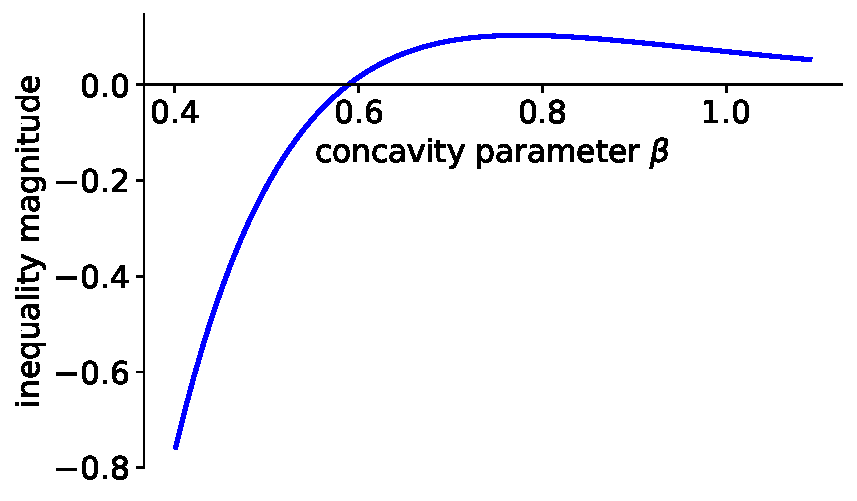
\includegraphics[width=.5\textwidth]{./chapter_real/figs/eta_constraint.pdf}
    \caption{\LHS of \eref{magnitude}. The inequality in \eref{magnitude} is 
    satisfied for any $\eta>0.589$, wherefore the choice that the subject made
    indicates that an ergodicity transformation with $\eta>.589$ is being optimised.
    For instance, this observation is consistent with a logarithmic ergodicity transformation ($\eta=1$).}
    \flabel{eta_constraint}
\end{SCfigure}

Each subject made 312 observed gambling choices. Each choice produces a similar statement -- some
constraint on $\eta$. 
Perhaps the next observation would show that the subject believes $\eta<1.2$, which would 
bracket the subject's belief about the value of $\eta $ into $0.589<\eta<1.2$. 

Like we said, the fitting techniques that were used to analyse the data from the experiment 
are quite sophisticated. Where inconsistencies in a subject's behaviours are observed, 
\eg of the type $\eta>0.589$ and $\eta<0.5$, this is interpreted 
as inaccuracy in the subject's estimate for $\eta$, in effect an inability of the subject to 
distinguish dynamics at this level of accuracy. The end result, after much computing, is a 
Bayesian posterior probability density function specifying the likelihood of a subject's beliefs
about $\eta$. Roughly, for each person in each environment this tells us how likely it is that the 
subject was optimizing expected changes in \eref{auto} with different values for $\eta$, \fref{HulmeETAL}.

For details, see \cite{MederETAL2019}. The statistical techniques used in the experiment
are described in \cite{LeeWagenmakers2013}.

%\begin{picture}(300,300)(-20,20)
%\put(-40,-20){\includegraphics[width=9.1cm]{./timeline.pdf}}
%\end{picture}

\begin{figure}
    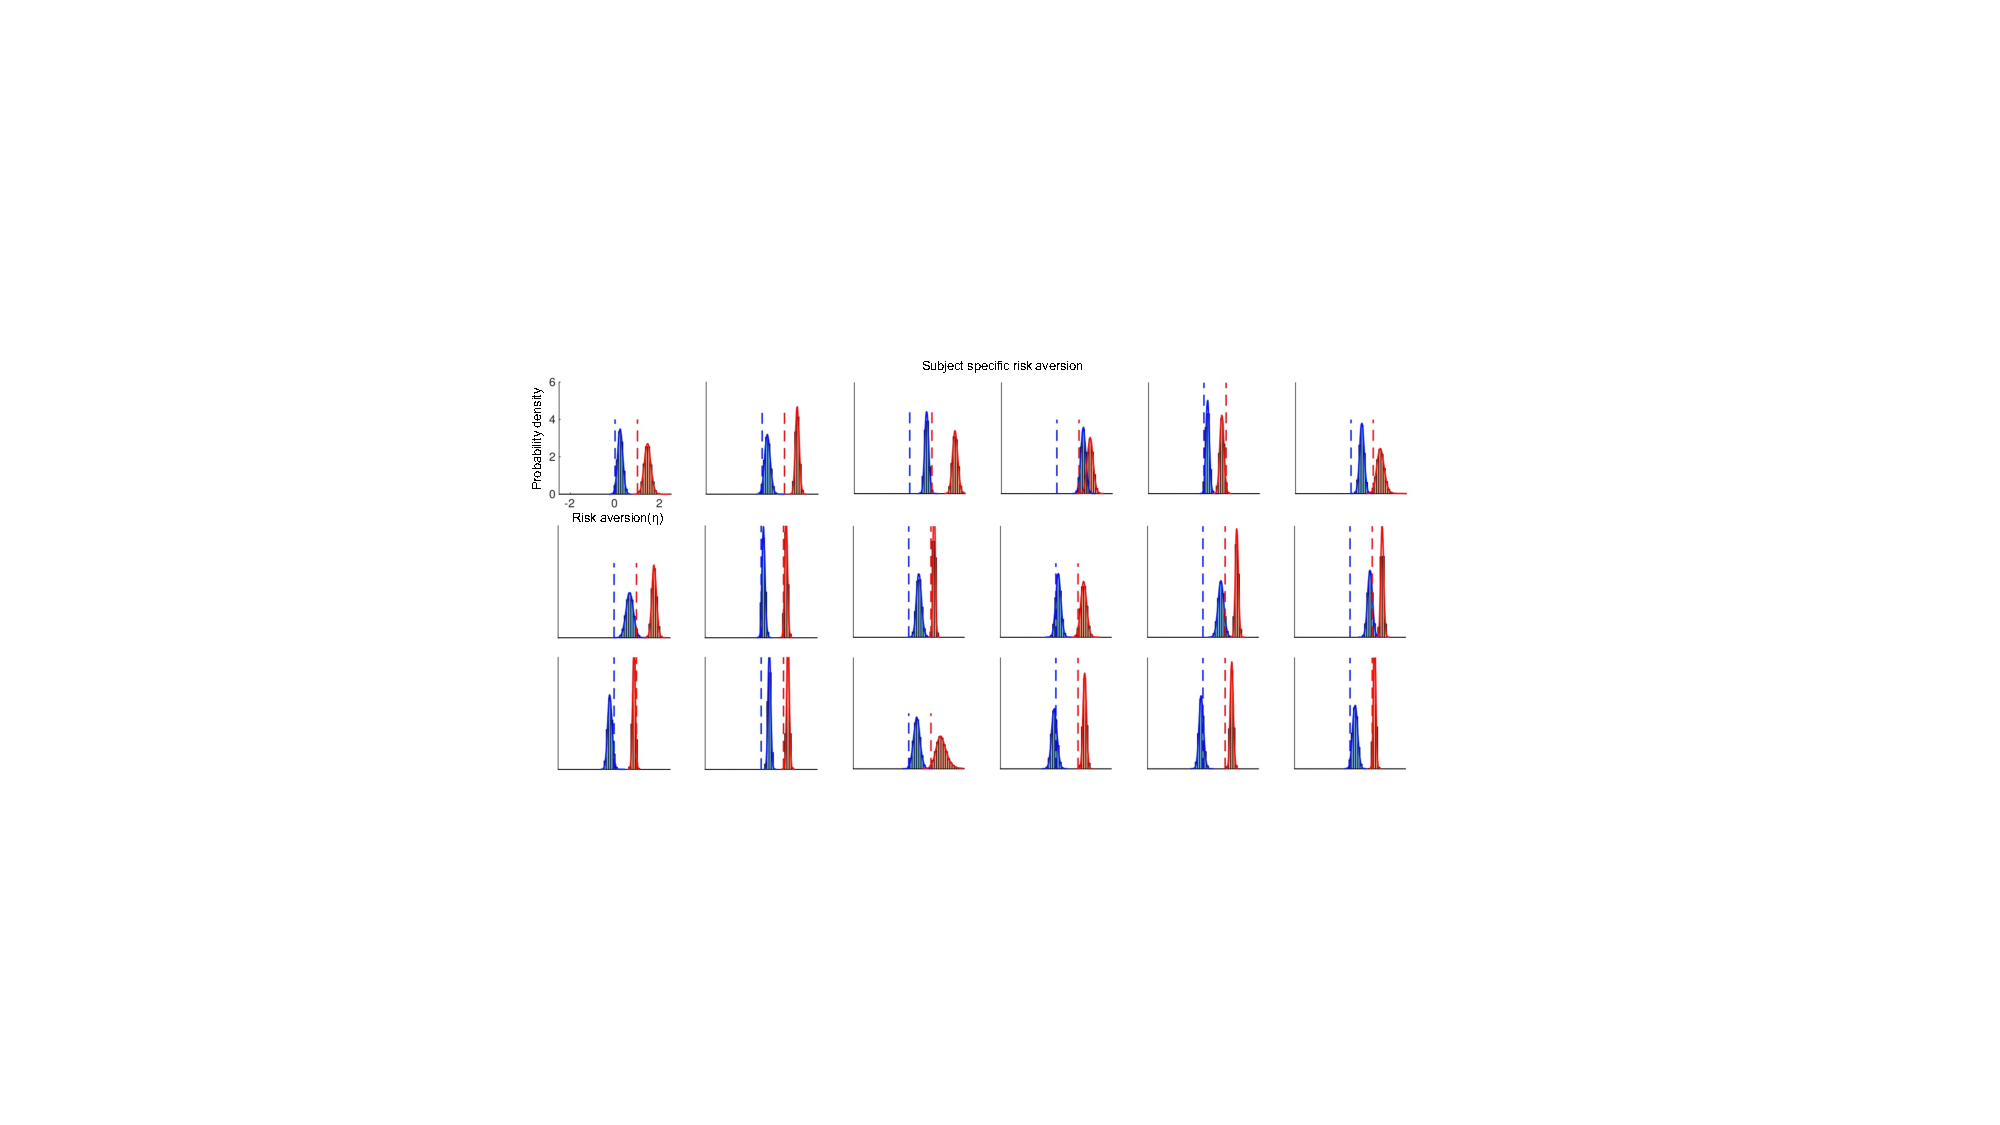
\includegraphics[width=\textwidth]{./chapter_real/singleSubjects.pdf}
    \caption{Posterior probability density functions for the parameter $\eta$ in the Copenhagen 
    experiment. Each panel is one individual, blue for the additive environment, red for 
    multiplicative. Dashed lines are the null-model predictions of 0 and 1. All tested individuals 
    changed behaviour noticeably in response to the wealth dynamic, in all cases the 
    multiplicative environment led to the shift to the right predicted by ergodicity economics. 
    Not all individuals are the same, but an overall pattern is clearly seen.}
    \label{fig:HulmeETAL}
\end{figure}

Expected-utility theory predicts that people are insensitive to changes in the dynamics. 
People may have wildly different utility functions, which would be reflected in wildly 
different best-fit values of $\eta$, but the dynamic setting should make no difference. 

Ergodicity economics predicts something quite different. First of all, it predicts that the 
dynamic setting significantly changes the best-fit ``utility function,'' which is really the 
ergodicity transformation in the relevant ergodic growth rate. The effective utility function will 
be different for one and the same individual under additive dynamics and under 
multiplicative dynamics. 

According to ergodicity economics, the direction of the change should go towards 
greater ``risk aversion'' for multiplicative dynamics -- the ergodicity mapping is more 
concave there. The magnitude of the change in $\eta$ should be about 1. And finally, 
if we take seriously the absolute null models of additive and multiplicative dynamics, 
the distributions should be centred near 0 for the additive setting and near 1 for the 
multiplicative setting. 
%This final prediction is unlikely to be borne out perfectly: what neuroscientists call ``bracketing'' -- the mental process of considering only the experiment, the game in front of us, and not our real-world situation -- is never quite perfect. This would suggest an overall shift towards greater risk aversion: real life is far more multiplicative than additive. Also, any uncertainty or doubt people may have about the setup are likely to translate into more cautious behaviour, another effect that would increase $\eta$ a little away from the null-model prediction.

Given the limitations of the experiment -- for instance people only had a one-hour 
training phase to get used to a given dynamic environment -- these predictions don't look 
so bad. Of course the 11,232 individual choices summarized in \fref{HulmeETAL} 
may be happenstance, or the experiment may be flawed in a way we don't yet 
understand. So we might put it this way: saying that expected-utility theory is 
based on good concepts corresponds to the belief that the difference between 
the red and blue curves is spurious.

\section{Insurance}
\seclabel{Insurance}
The insurance contract is an important and ubiquitous type of economic transaction, 
which can be modelled as a gamble. Its significance is two-fold: insurance contracts 
transfer risk from one party to another, and this -- the transfer, or sharing, of risk -- is 
a key driver of the emergence of social structure at all levels of evolution 
\secref{Cooperation}. More mundanely, insurance is an important thing
to understand because the selling and buying of insurance contracts (derivatives)
constitutes the vast majority of global trade. Perhaps -- a tantalising hypothesis -- 
these two facts are not unrelated.

However, classically insurance poses a puzzle~\cite{PetersAdamou2015b}. In 
the expected-wealth paradigm, insurance contracts shouldn't exist, because 
buying insurance would only be rational at a price at which it would be irrational 
to sell. More specifically:
\begin{enumerate}
\item To be viable, an insurer must charge an insurance premium of at least the 
expectation value of any claims that may be made against it, called the ``net 
premium'' \cite[p.~1]{KaasETAL2008}.
\item The insurance buyer therefore has to be willing to pay more than the expectation
value of the claims he will receive (the net premium), so that an insurance contract 
may be successfully signed.
\item Under the expected-wealth paradigm it is irrational to pay more than the 
net premium, and therefore insurance contracts should not exist.
\end{enumerate}
In this picture, an insurance contract can only ever be beneficial to one party. It 
has the anti-symmetric property that the expectation value of one party's gain is 
the expectation value of the other party's loss.

The puzzle is that insurance contracts are observed to exist. Why? Classical 
resolutions appeal to utility 
theory (\ie psychology) and asymmetric information (\ie deception). However, 
ergodicity economics naturally predicts contracts with a range of prices that 
increase the time-average growth rate for both buyer and seller. 
This is rather an important point. It means that, at a good price, insurance 
contracts are mutually beneficial -- a theme we will return to in \secref{Cooperation}. 
We will also see that these voluntary contracts lead to a flow of cash from 
poor to rich -- another theme we will return to, in \secref{Reallocation}.

We illustrate how this all works with an example drawn from maritime trade, in 
which the use of insurance 
has a very long history.\footnote{Contracts between Babylonian traders and 
lenders were recorded around 1750 BC in the Code of Hammurabi. Chinese 
traders practised diversification by spreading cargoes across multiple vessels 
even earlier than this, in the third millennium BC.} A similar 
example was used by Bernoulli~\cite{Bernoulli1738}, incidentally in the
paper containing his solution to the St. Petersburg paradox.

\section{Setup: a shipping insurance contract}
We imagine a shipowner sending cargo from St Petersburg to Amsterdam, 
with the following parameters:
\begin{itemize}
\item owner's wealth, $\x_\text{own}=\$100,000$;
\item gain on safe arrival of cargo, $\G=\$4,000$;
\item probability ship will be lost, $\p=0.05$;
\item replacement cost of the ship, $\C=\$30,000$; and
\item voyage time, $\dt=1$ month.
\end{itemize}
An insurer with wealth $\x_\text{ins}=\$1,000,000$ proposes to insure the voyage for a 
fee, $\F=\$1,800$. If the ship is lost, the insurer pays the owner $\gL=\G+\C$ to make him 
good on the loss of his ship and the profit he would have made.

We phrase the decision the owner is facing as a choice between 
two gambles. 

\begin{definition}{The owner's gambles}

Sending the ship uninsured corresponds to gamble o1
\bea
\q_1^{(\text{o1})} = \G, &\quad& \p_1^{(\text{o1})} = 1-p;\\
\q_2^{(\text{o1})} = -\C, &\quad& \p_2^{(\text{o1})} = p.
\eea
Sending the ship fully insured corresponds to gamble o2
\bea
\q_1^{(\text{o2})} = \G-\F &\quad& \p_1^{(\text{o2})} = 1.
\eea
This is a trivial ``gamble'' because all risk has been 
transferred to the insurer. 
\end{definition}

We also model the insurer's decision whether to offer the contract as
a choice between two gambles

\begin{definition}{The insurer's gambles}

Not insuring the ship corresponds to gamble i1, which is the null gamble
\bea
\q_1^{(\text{i1})} = 0 &\quad& \p_1^{(\text{i1})} = 1.
\eea

Insuring the ship corresponds to gamble i2
\bea
\q_1^{(\text{i2})} = +\F, &\quad& \p_1^{(\text{i2})} = 1-p;\\
\q_2^{(\text{i2})} = -\gL+\F, &\quad& \p_2^{(\text{i2})} = p.
\eea
\end{definition}

To establish the puzzle, we ask in the expected-wealth paradigm whether 
the owner should sign the contract, and whether the insurer should have proposed it.

\subsubsection{Insurance in the expected-wealth paradigm}
In the expected-wealth paradigm (corresponding to additive repetition under 
the time paradigm) decision makers
maximise the rate of change of the expectation values of their wealths, according to \eref{ex_crit}:
Under this paradigm the owner collapses gamble o1 into the scalar

\bea
\gt_a^{(\text{o1})} &=& \frac{\ave{\d\x}}{\dt}\\
&=&\frac{\ave{\q^{(\text{o1})}}}{\dt}\\
&=&\frac{(1-p) \G + p (-\C) }{\dt}\\
&=&\$ 2,300\text{ per month,}
\eea

and gamble o2 into the scalar

\bea
\gt_a^{\text{o2}} &=&\frac{\ave{\q^{(\text{o2})}}}{\dt}\\
&=&\frac{(\G-\F) }{\dt}\\
&=&\$2,200 \text{ per month.}
\eea
The difference, $\delta\gt_a^\text{o}$,  between the expected rates 
of change in wealth with and without a signed contract is the expected 
loss minus the fee per round trip,
\be
\delta\gt_a^\text{o}=\gt_a^{\text{o2}}-\gt_a^{\text{o1}}= \frac{\p \gL - \F}{\dt}.
\elabel{dro}
\ee
The sign of this difference indicates whether the insurance contract is beneficial
to the owner. In the example this is not the case, $\delta\gt_a^\text{o}=-\$100$ per month.

The insurer evaluates the gambles i1 and i2 similarly, with the result
\be
\gt_a^{(\text{i1})}  = \$0 \text{ per month,}
\ee
and
\bea
\gt_a^{(\text{i2})}  &=& \frac{\F-\p \gL}{\dt} \elabel{r}\\ 
&=& \$100 \text{ per month.}
\eea
Again we compute the difference -- the net benefit to the insurer that arises from signing the contract
\be
\delta\gt_a^\text{i}=\gt_a^{\text{i2}}-\gt_a^{\text{i1}}= \frac{\F- \p \gL}{\dt}.
\elabel{dri}
\ee
In the example this is $\delta\gt_a^\text{i}=\$100$ per month, meaning that in the 
world of the expected-wealth paradigm the insurer will offer the contract.


Because only one party (the insurer) is willing to sign, no contract will come into existence. We could think that we got
the price wrong, and the contract would be signed if offered at a different fee. 
But this is not the case. Looking at \eref{dro} and \eref{dri} we notice the anti-symmetric 
relationship between the two expressions, 
\be
\delta\gt_a^\text{o}=-\delta\gt_a^\text{i}.
\ee
By symmetry, there can be no fee at which both expressions are positive. 
If one is positive, the other must be negative. The only point where this
isn't the case is when both sides are exactly zero.
Hence there are no circumstances in the world created by the 
expected-wealth paradigm under which both parties have an incentive to 
sign; there is merely one specific price at which neither party has a reason 
to refrain from signing. Insurance contracts cannot exist in this model world.

\begin{keypts}{Fundamental insurance puzzle}
In the model world created by expected-wealth maximisation, {\it no price exists} at 
which two parties will sign an insurance contract.
\end{keypts}

One party winning at the expense of the other makes insurance an 
unsavoury business in the expected-wealth paradigm. This is further 
illustrated in \fref{ins_lin}, which shows the change in the rate of 
change of expected wealth (the decision criterion) for both parties 
as a function of the fee, $\F$.
\begin{SCfigure}
\centering
%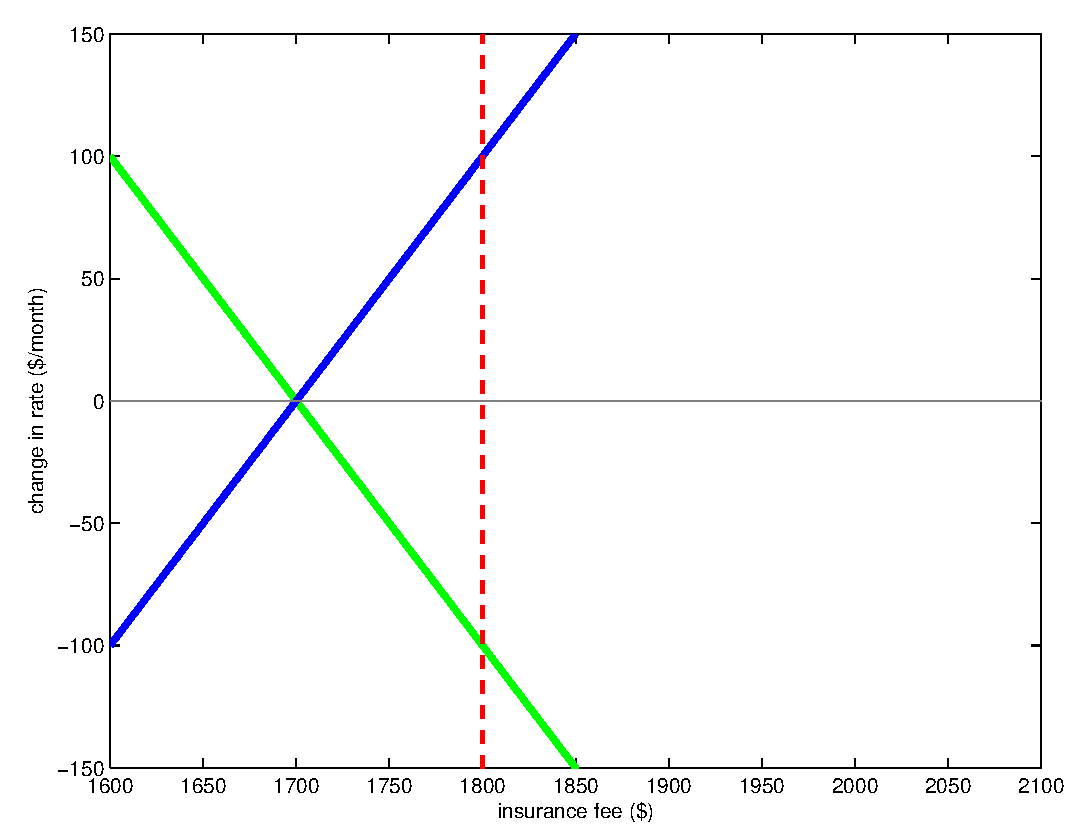
\includegraphics[width=.5\textwidth]{./chapter_riskless/figs/ins_lin_cropped.pdf}
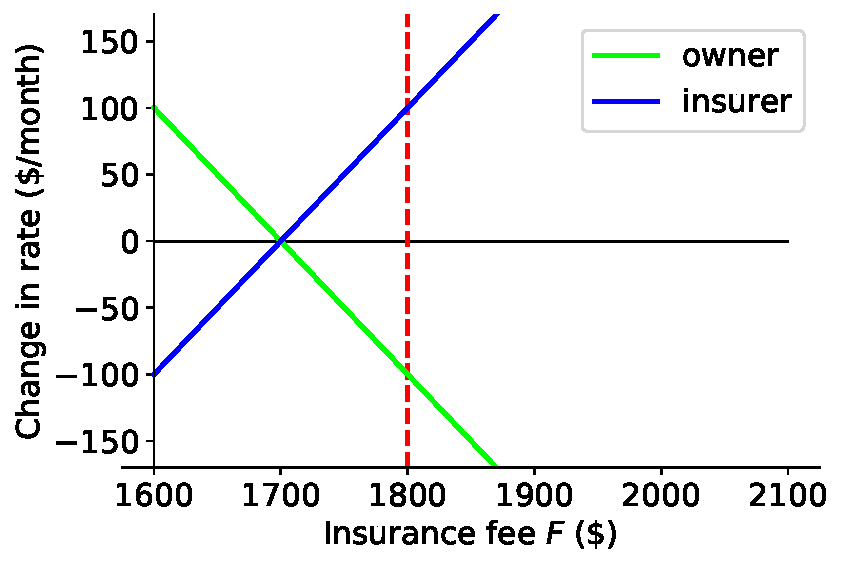
\includegraphics[width=.5\textwidth]{./chapter_real/figs/insurance_exp.pdf}
\caption{Change in the rate of change of expected wealth for the shipowner (green) and the 
insurer (blue) as a function of the insurance fee, $\F$.\flabel{ins_lin}}
\end{SCfigure}
There is no price at which the decision variable is positive for both parties. The best they can 
do is to pick the price at which neither of them cares whether they sign or not.

In this picture, the existence of insurance contracts requires some asymmetry 
between the contracting parties, such as:
\begin{itemize}
\item different psychological attitudes to bearing risk;
\item different access to information about the voyage;
\item different assessments of the riskiness of the voyage;
\item one party to deceive, coerce, or gull the other into a bad decision.
\end{itemize}
It is difficult to believe that this is truly the basis for a market of the size and 
global reach of the insurance market.

\subsection{Ergodicity economics solution}

Ergodicity economics resolves the insurance puzzle under many
different types of dynamics -- so long as the ergodicity mapping is
concave. For simplicity we will assume multiplicative dynamics, pausing 
to reflect on the difference to additive dynamics (which is equivalent to 
the expected-wealth paradigm that created the insurance puzzle). 
Assuming a multiplicative wealth dynamic models the 
ship owner as sending out a ship and a cargo whose values are proportional to 
his wealth at the start of each voyage. A rich owner who has had many 
successful voyages will send out more cargo, a larger ship, or perhaps a 
\textit{flotilla}, while an owner to whom the sea has been a cruel mistress 
will send out a small vessel until his luck changes. Modelling wealth with an
additive dynamic, the ship owner would send out the same amount
of cargo on each journey, irrespective of his wealth. Shipping companies
of the size of Evergreen or Maersk would be inconceivable under additive 
dynamics, where returns on successful investments are not reinvested.

Under multiplicative dynamics, the two parties seek to maximise
\be
\gt_m = \lim_{\Dt\to\infty}\frac{\D\gv(\x)}{\Dt} = \frac{\ave{\d\ln \x}}{\dt},
\ee
where we have used the ergodic property of $\D\gv(\x)=\D\ln\x$.

The owner's time-average growth rate without insurance is 
\be
\gt_m^\text{o1} = \frac{(1-\p)\ln(\x_\text{own}+\G)+\p\ln(\x_\text{own}-\C) - \ln(\x_\text{own})}{\dt}
\ee
or 1.9\% per month. 
His time-average growth rate with insurance is 
\be
\gt_m^\text{o2} = \frac{\ln(\x_\text{own}+\G-\F)-\ln(\x_\text{own})}{\dt}
\ee
or 2.2\% per month. This gives a net benefit for the owner of
\be
\d\gt_m^o = \gt_m^\text{o2}-\gt_m^\text{o1} \approx +0.24\% \text{ per month.} 
\ee
The time paradigm thus creates a world where the owner will sign the contract.

What about the insurer? Without insurance, the insurer plays the null gamble, and
\be
\gt_m^{\text{i1}}= \frac{0}{\dt}
\ee
or 0\% per month. His time-average growth rate with insurance is 
\be
\gt_m^{\text{i2}} = \frac{(1-p)\ln(\x_\text{ins}+\F) + p\ln(\x_\text{ins}+\F-\gL) - \ln(\x_\text{ins})}{\dt}
\ee
or 0.0071\% per month. The net benefit to the insurer is therefore also
\be
\delta\gbar_m^{\text{i}} = \gt_m^{\text{i2}}-\gt_m^{\text{i1}}
\ee
\ie 0.0071\% per month. Unlike the expected wealth paradigm, ergodicity economics 
with multiplicative repetition creates a world where an insurance contract can exist -- 
there exists a range of fees $\F$ at which both parties gain from signing the contract! 

We view this as the fundamental resolution of the insurance puzzle.
\begin{keypts}{Fundamental resolution of the insurance puzzle:}
An insurance contract will be signed by both parties if doing so 
increases the time-average ergodic growth rate
of both the seller's wealth and the buyer's wealth.
\end{keypts}
It requires no appeal to arbitrary utility functions or asymmetric circumstances, rather 
it arises naturally from the model of human decision-making that we have set out. 
\fref{ins_log} shows the mutually beneficial range of insurance fees predicted by our model.
\begin{SCfigure}
\centering
%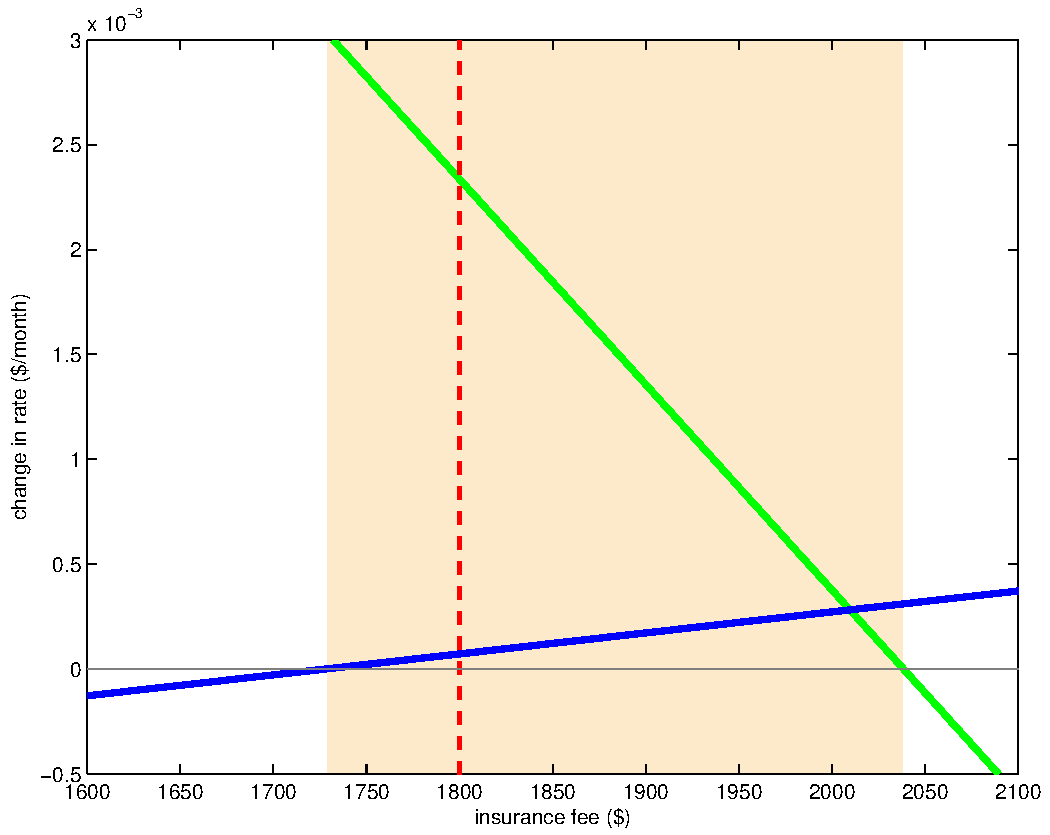
\includegraphics[width=.5\textwidth]{./chapter_riskless/figs/ins_log_cropped.pdf}
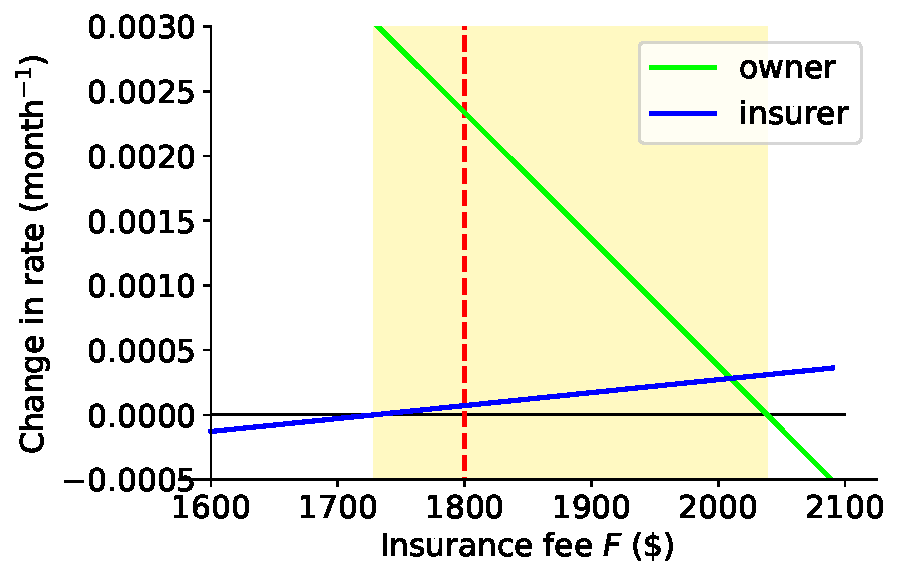
\includegraphics[width=.5\textwidth]{./chapter_real/figs/insurance_erg.pdf}
\caption{Change in the time-average growth rate of wealth for the shipowner (green) and the insurer 
(blue) as a function of the insurance fee, $F$. The mutually beneficial fee range is marked by the beige background.\flabel{ins_log}}
\end{SCfigure}

Generalizing, the message of ergodicity economics is that business happens when both parties gain.
In the world created by this model any agreement, any contract, any commercial interaction 
comes into existence because it is mutually beneficial.

%\printglossary[title=Glossary,type=\acronymtype]
%%
%\printglossary[title=List of Symbols]
\subsection{The classical solution of the insurance puzzle}
\seclabel{The classical solution of the insurance puzzle}

%\begin{example}{Expected-utility paradigm}
%Let's look at the solution in the expected-utility paradigm. Our players now seek to maximise the rate of change of their expected utility,
%\be
%\ave{r_u} \equiv \frac{\ave{\Du(W)}}{\Dt}.
%\ee
%To make the example concrete, we will use $u(W)=\sqrt{W}$, as suggested by Cramer~\cite{Cramer1728}, for both parties.
%
%The owner has
%\be
%\ave{r_u}_\text{own}^\text{un} = \frac{(1-p)u(W_\text{own}+G)+pu(W_\text{own}-C) - u(W_\text{own})}{\Dt}
%\ee
%or 3.37 `utils'\footnotemark\ per month without insurance, and 
%\be
%\ave{r_u}_\text{own}^\text{in} = \frac{u(W_\text{own}+G-F)-u(W_\text{own})}{\Dt}
%\ee
%or 3.46 utils per month with insurance. The change in $\ave{r_u}_\text{own}$ is 
%\be
%\delta\ave{r_u}_\text{own} = \ave{r_u}_\text{own}^\text{in} - \ave{r_u}_\text{own}^\text{un},
%\ee
%\ie 0.094 utils per month, and the owner should sign.
%
%The contract is also favourable from the insurer's perspective. If he does no business, then 
%\be
%\ave{r_u}_\text{ins}^\text{un} = \frac{0}{\Dt}
%\ee
%or zero utils per month. If he extends insurance, then
%\be
%\ave{r_u}_\text{ins}^\text{in} = \frac{(1-p)u(W_\text{ins}+F) + pu(W_\text{ins}+F-L) - u(W_\text{ins})}{\Dt}
%\ee
%or 0.043 utils per month and his change in $\ave{r_u}_\text{ins}$ is positive:
%\be
%\quad \delta\ave{r_u}_\text{ins} = \ave{r_u}_\text{ins}^\text{in} - \ave{r_u}_\text{ins}^\text{un},
%\ee
%\ie 0.043 utils per month.
%\end{example}
%\footnotetext{The general unit of utility. Here $1\,\text{util} = \sqrt{\$}\,1$, whatever that might mean.}
The classical solution of the insurance puzzle is identical to the classical solution of the St Petersburg paradox.
Wealth is replaced by a non-linear utility function of wealth, which breaks the symmetry of the 
expected-wealth paradigm. While it is always true that $\delta\ave{r}_\text{own}=-\delta\ave{r}_\text{ins}$, 
the expected growth rates of non-linear utility functions don't share this anti-symmetry. A difference in 
the decision makers' wealths is sufficient, though often different utility functions are assumed for owner and insurer, 
which is a model that can create pretty much any behaviour. The downside of a model with this ability is, of course, 
that it makes no predictions -- nothing is ruled out, so the model cannot be falsified. Popper would mark it as 
not science.
%
%This represents the classical resolution of the insurance puzzle. The symmetry broken by the different wealths $W_\text{own}$ and $W_\text{ins}$, which now appear in $\ave{r_u}$ since the utility function is nonlinear.\footnote{Note that the symmetry could also have been broken by assigning different utility functions to the two parties, even if their wealths were the same. However, it suffices only that their wealths be different for the puzzle to be resolved.} Certain combinations of $W_\text{own}$, $W_\text{ins}$, and $u$ will admit a range of mutually beneficial prices, $F$. This is visible as the beige region in \fref{ins_sqrt}, which plots the decision variable, $\delta\ave{r_u}$, for both parties as a function of the fee, $F$.
%\begin{figure}
%\centering
%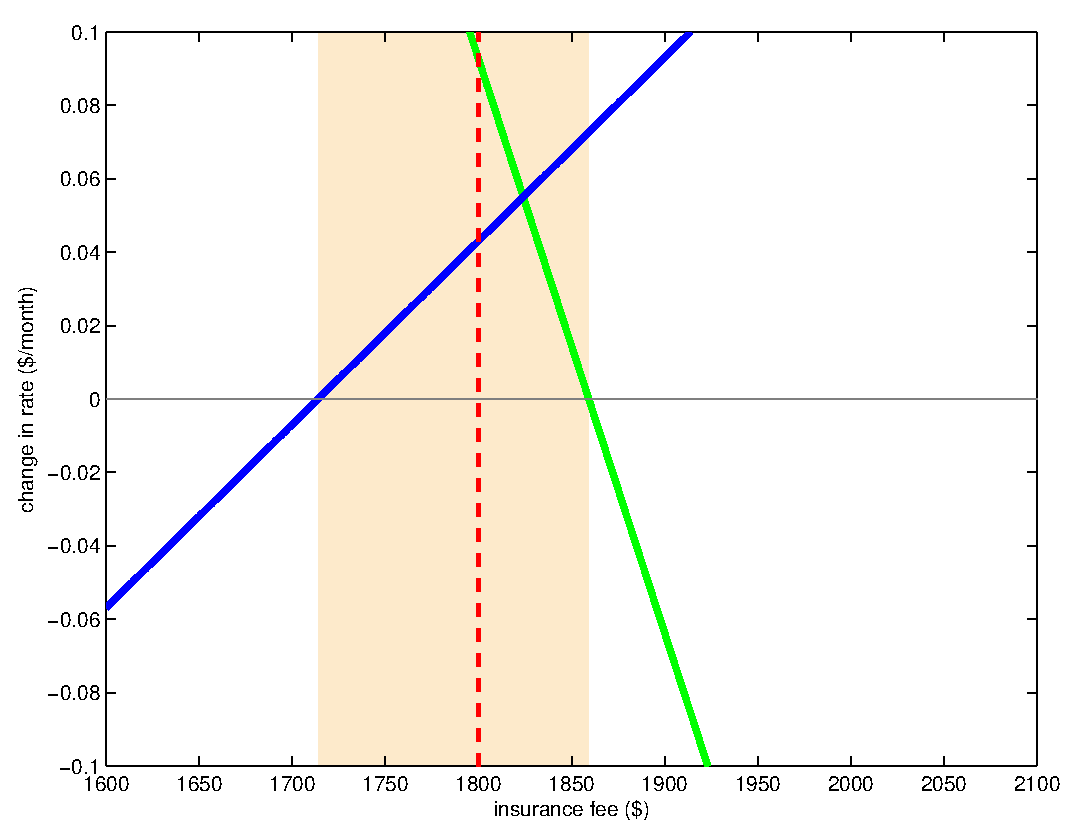
\includegraphics[width=\textwidth]{./chapter_riskless/figs/ins_sqrt_cropped.pdf}
%\caption{Change in the rate of change of expected square-root utility for the shipowner (green) and the insurer (blue) as a function of the insurance fee, $F$. The mutually beneficial fee range is marked by the beige background.\flabel{ins_sqrt}}
%\end{figure}
%Utility theory does not rule out insurance contracts -- it is {\it possible} to create a win-win deal -- but does not rule them in either. Furthermore, invoking arbitrary and unobservable utility functions hardly seems a satisfying resolution of the puzzle.